\clearpage
\VerdierPhysicalPageAnchor{0091}%
\VerdierSemanticAnchor{ch1-3-2-8-j-induced-functorial-map}
态射 $J\colon c(p(f))\longrightarrow X[1]$ 对应于如下函子态射，
这一点可立即验证：

\VerdierSemanticAnchor{ch1-3-2-8-eq3}
\begin{equation}
  \begin{gathered}
    D=
    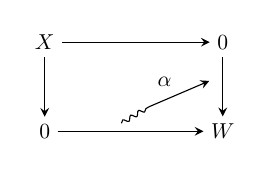
\begin{tikzpicture}[>=stealth,baseline=(current bounding box.center),
      scale=0.78,every node/.style={transform shape}]
      \node (X)  at (0,1.45) {$X$};
      \node (Z1) at (2.9,1.45) {$0$};
      \node (Z2) at (0,0) {$0$};
      \node (W)  at (2.9,0) {$W$};
      \draw[->] (X) -- (Z1);
      \draw[->] (X) -- (Z2);
      \draw[->] (Z1) -- (W);
      \draw[->] (Z2) -- (W);
      \draw[decorate,decoration={snake,amplitude=0.8pt,segment length=3.3pt}]
        (1.25,0.13) -- (1.70,0.40);
      \draw[->] (1.70,0.40) -- node[above left] {$\alpha$} (2.68,0.82);
    \end{tikzpicture}
    \quad\longmapsto\quad
    JD=\bigl(0\colon Y\longrightarrow W,\;
      0\colon0\rightsquigarrow0,\;
      \alpha\colon0\rightsquigarrow0\bigr).
  \end{gathered}
  \tag{3.2.8.3}
\end{equation}

\VerdierSemanticAnchor{ch1-3-2-8-h-induced-functorial-map}
依定义 (3.2.7)，态射 $H\colon X[1]\longrightarrow c(p(f))$
对应于如下函子态射：

\VerdierSemanticAnchor{ch1-3-2-8-eq4}
\begin{equation}
  \begin{aligned}
    t={}&\bigl(m\colon Y\longrightarrow W,\;
      a\colon0\rightsquigarrow m,\;
      b\colon0\rightsquigarrow mf\bigr)\\[-0.2em]
    &\longmapsto\quad Ht=
    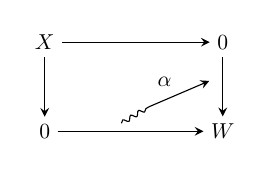
\begin{tikzpicture}[>=stealth,baseline=(current bounding box.center),
      scale=0.78,every node/.style={transform shape}]
      \node (X)  at (0,1.45) {$X$};
      \node (Z1) at (2.9,1.45) {$0$};
      \node (Z2) at (0,0) {$0$};
      \node (W)  at (2.9,0) {$W$};
      \draw[->] (X) -- (Z1);
      \draw[->] (X) -- (Z2);
      \draw[->] (Z1) -- (W);
      \draw[->] (Z2) -- (W);
      \draw[decorate,decoration={snake,amplitude=0.8pt,segment length=3.3pt}]
        (1.25,0.13) -- (1.70,0.40);
      \draw[->] (1.70,0.40) -- node[above left] {$\alpha$} (2.68,0.82);
    \end{tikzpicture}
    ,\qquad \alpha=b-a\star f.
  \end{aligned}
  \tag{3.2.8.4}
\end{equation}

\VerdierSemanticAnchor{ch1-3-2-8-composite-identity}
这两个函子态射的复合确为恒等，从而证明了断言 (3.2.7.2)。

\VerdierSemanticAnchor{ch1-3-2-9}
\noindent\textbf{3.2.9. 断言 (3.2.7.3) 的证明。}\quad
\VerdierSemanticAnchor{ch1-3-2-9-hj-functorial-map}
由 (3.2.8)，态射
$HJ\colon c(p(f))\longrightarrow c(p(f))$ 对应于如下函子态射：

\VerdierSemanticAnchor{ch1-3-2-9-eq1}
\begin{equation}
  \begin{aligned}
    t={}&\bigl(m\colon Y\longrightarrow W,\;
      a\colon0\rightsquigarrow m,\;
      b\colon0\rightsquigarrow mf\bigr)
      \longmapsto HJt\\
    ={}&\bigl(0\colon Y\longrightarrow W,\;
      0\colon0\rightsquigarrow0,\;
      b-a\star f\colon0\rightsquigarrow0\bigr)
  \end{aligned}
  \tag{3.2.9.1}
\end{equation}
因此：

\VerdierSemanticAnchor{ch1-3-2-9-eq2}
\begin{equation}
  t-HJt=\bigl(m\colon Y\longrightarrow W,\;
    a\colon0\rightsquigarrow m,\;
    a\star f\colon0\rightsquigarrow mf\bigr).
  \tag{3.2.9.2}
\end{equation}

\VerdierSemanticAnchor{ch1-3-2-9-null-homotopy-reduction}
为证明断言 (3.2.7.3)，只需证明每个形如
$\bigl(m\colon Y\longrightarrow W,\;a\colon0\rightsquigarrow m,\;
a\star f\colon0\rightsquigarrow mf\bigr)$ 的三元组，都对应于一个从
$c(p(f))$ 到 $W$ 的同伦于零的态射。利用 (3.1.3)，这样的三元组定义一个态射：

\VerdierSemanticAnchor{ch1-3-2-9-eq3}
\begin{equation}
  v\colon c(f)\longrightarrow W,
  \qquad
  v=\bigl(m\colon Y\longrightarrow W,\;
    a\star f\colon0\rightsquigarrow mf\bigr)
  \tag{3.2.9.3}
\end{equation}
以及一个同伦：

\VerdierSemanticAnchor{ch1-3-2-9-eq4}
\begin{equation}
  a\colon0\rightsquigarrow vp(f)=m,
  \tag{3.2.9.4}
\end{equation}
